%!TEX root = main.tex

\section{Data}\label{sec:data}


{\bf(I just realized that “full” sample is in the data section as meaning something other than the “full matched” sample in the results section - you need to decide on a consistent naming convention that is clear and unambiguous and change the text throughout.  Maybe ``full'' sample in the data section and ``matched'' sample in the results section?)}

In this section we describe the PRIMUS redshift survey data, how we identify star-forming
and quiescent galaxies, and how we define the isolated primary samples used to measure 
the conformity signal within PRIMUS.

%low-resolution ($\lambda/\Delta\lambda \sim 40$) spectra for $\sim$300,000 objects
%targeted $80\%$ of galaxies in these fields with $i < 22$
%IMACS instrument \citep{Bigelow03} on Magellan-I Baade 6.5 m telescope to observe $\sim$2,500 objects at once using a slitmask that covered 0.18~$\degsq$
%statistically-complete sample of $\sim$120,000 spectroscopic redshifts to $i_{\mathrm{AB}}\sim23.5$
%redshifts are derived by fitting a large suite of galaxy, broad-line AGN, and stellar spectral templates to the low-resolution spectra and optical photometry \citep[see][for details]{Cool13}
%objects are classified as galaxies, broad-line AGN or stars depending on the best $\chi^2$ template fit
%redshift precision is ($\sigma_z/(1+z) \sim 0.5\%$)
%low catastrophic outlier rate: less than $3\%$ ($\Delta{z}/(1+z) \ge 0.03$)
%further details of the survey design, targeting, and data see \citet{Coil11}
%further details of the data reduction, redshift confidence, and completeness see \citet{Cool13}

\subsection{PRIMUS}\label{sec:PRIMUS}
 
The PRIsm MUlti-Object Survey (PRIMUS) is the largest spectroscopic faint galaxy redshift survey completed to date.
The survey was conducted with the IMACS spectrograph (Bigelow \& Dressler 2003) on the Magellan I Baade 6.5-meter telescope at 
Las Campanas 
Observatory, using slitmasks and low-dispersion prism.
The design allowed for $\sim$2,000 objects per slitmask to be observed simultaneously with a spectral resolution of ${\lambda/\Delta
\lambda \sim 40}$, in 
a field of view of $\sim$0.2~$\degsq$.
Objects were targeted to a maximum depth of ${i \ge 23}$, and typically two slitmasks were observed per pointing on the sky.  
PRIMUS obtained robust redshifts $({Q \ge 3}$, see \citet{Coil11} and \citet{Cool13}, for $\sim$120,000 objects at ${z \sim 
0\textendash1.2}$ with a 
redshift precision of ${\sigma_{z}/(1 + z) \sim 0.005}$.

The total survey area of PRIMUS is $9.1~\degsq$ and encompasses seven distinct science fields:
the Chandra Deep Field South-SWIRE field \citep[CDFS;][]{Lonsdale03},
the 02hr and 23hr DEEP2 fields \citep{Newman13},
the COSMOS field \citep{Scoville07},
the European Large Area ISO Survey-South 1 field \citep[ES1;][]{Oliver00},
the Deep Lens Survey \citep[DLS;][]{Wittman02} F5 field,
and two spatially adjacent subfields of the XMM-Large Scale Structure Survey field \citep[XMM-LSS;][]{Pierre04}.
The XMM subfields are the Subaru/XMM-Newton DEEP Survey field \citep[XMM-SXDS;][]{Furusawa08} and the Canada-France-Hawaii 
Telescope Legacy 
Survey (CFHTLS) field (XMM-CFHTLS).
These two fields are adjacent but are treated separately in our analysis 
as they were targeted by PRIMUS using different photometric catalogs \citep[see][for details]{Coil11}.
%PRIMUS also includes an additional four calibration fields that had prior, high resolution spectroscopic redshifts.
Full details of the survey design, targeting, and data summary can be found in \citet{Coil11}, white details the of data reduction, redshift 
fitting, precision, 
and survey completeness are available in \citet{Cool13}.

Here we use the PRIMUS fields that have deep multi-wavelength ultraviolet (UV) imaging from the Galaxy Evolution Explorer 
\citep[GALEX;][]{Martin05}, 
mid-infrared imaging from the Spitzer Space Telescope \citep{Werner04} Infrared Array Camera \citep[IRAC;][]{Fazio04}, and optical and 
near-IR imaging 
from various ground-based surveys.
They include the CDFS, COSMOS, ES1, XMM-CFHTLS, and XMM-SXDS fields, covering {$\sim$5.5~$\degsq$} on the sky.

\begin{figure*}
  \centering
%  \epsscale{1.0}
%  \epstrim{0.0in 0.5in 0.2in 0.6in}
%  \fbox{\plotone{figures/cone_diagrams}}
%  \plotone{figures/cone_diagrams.eps}
%  \fbox{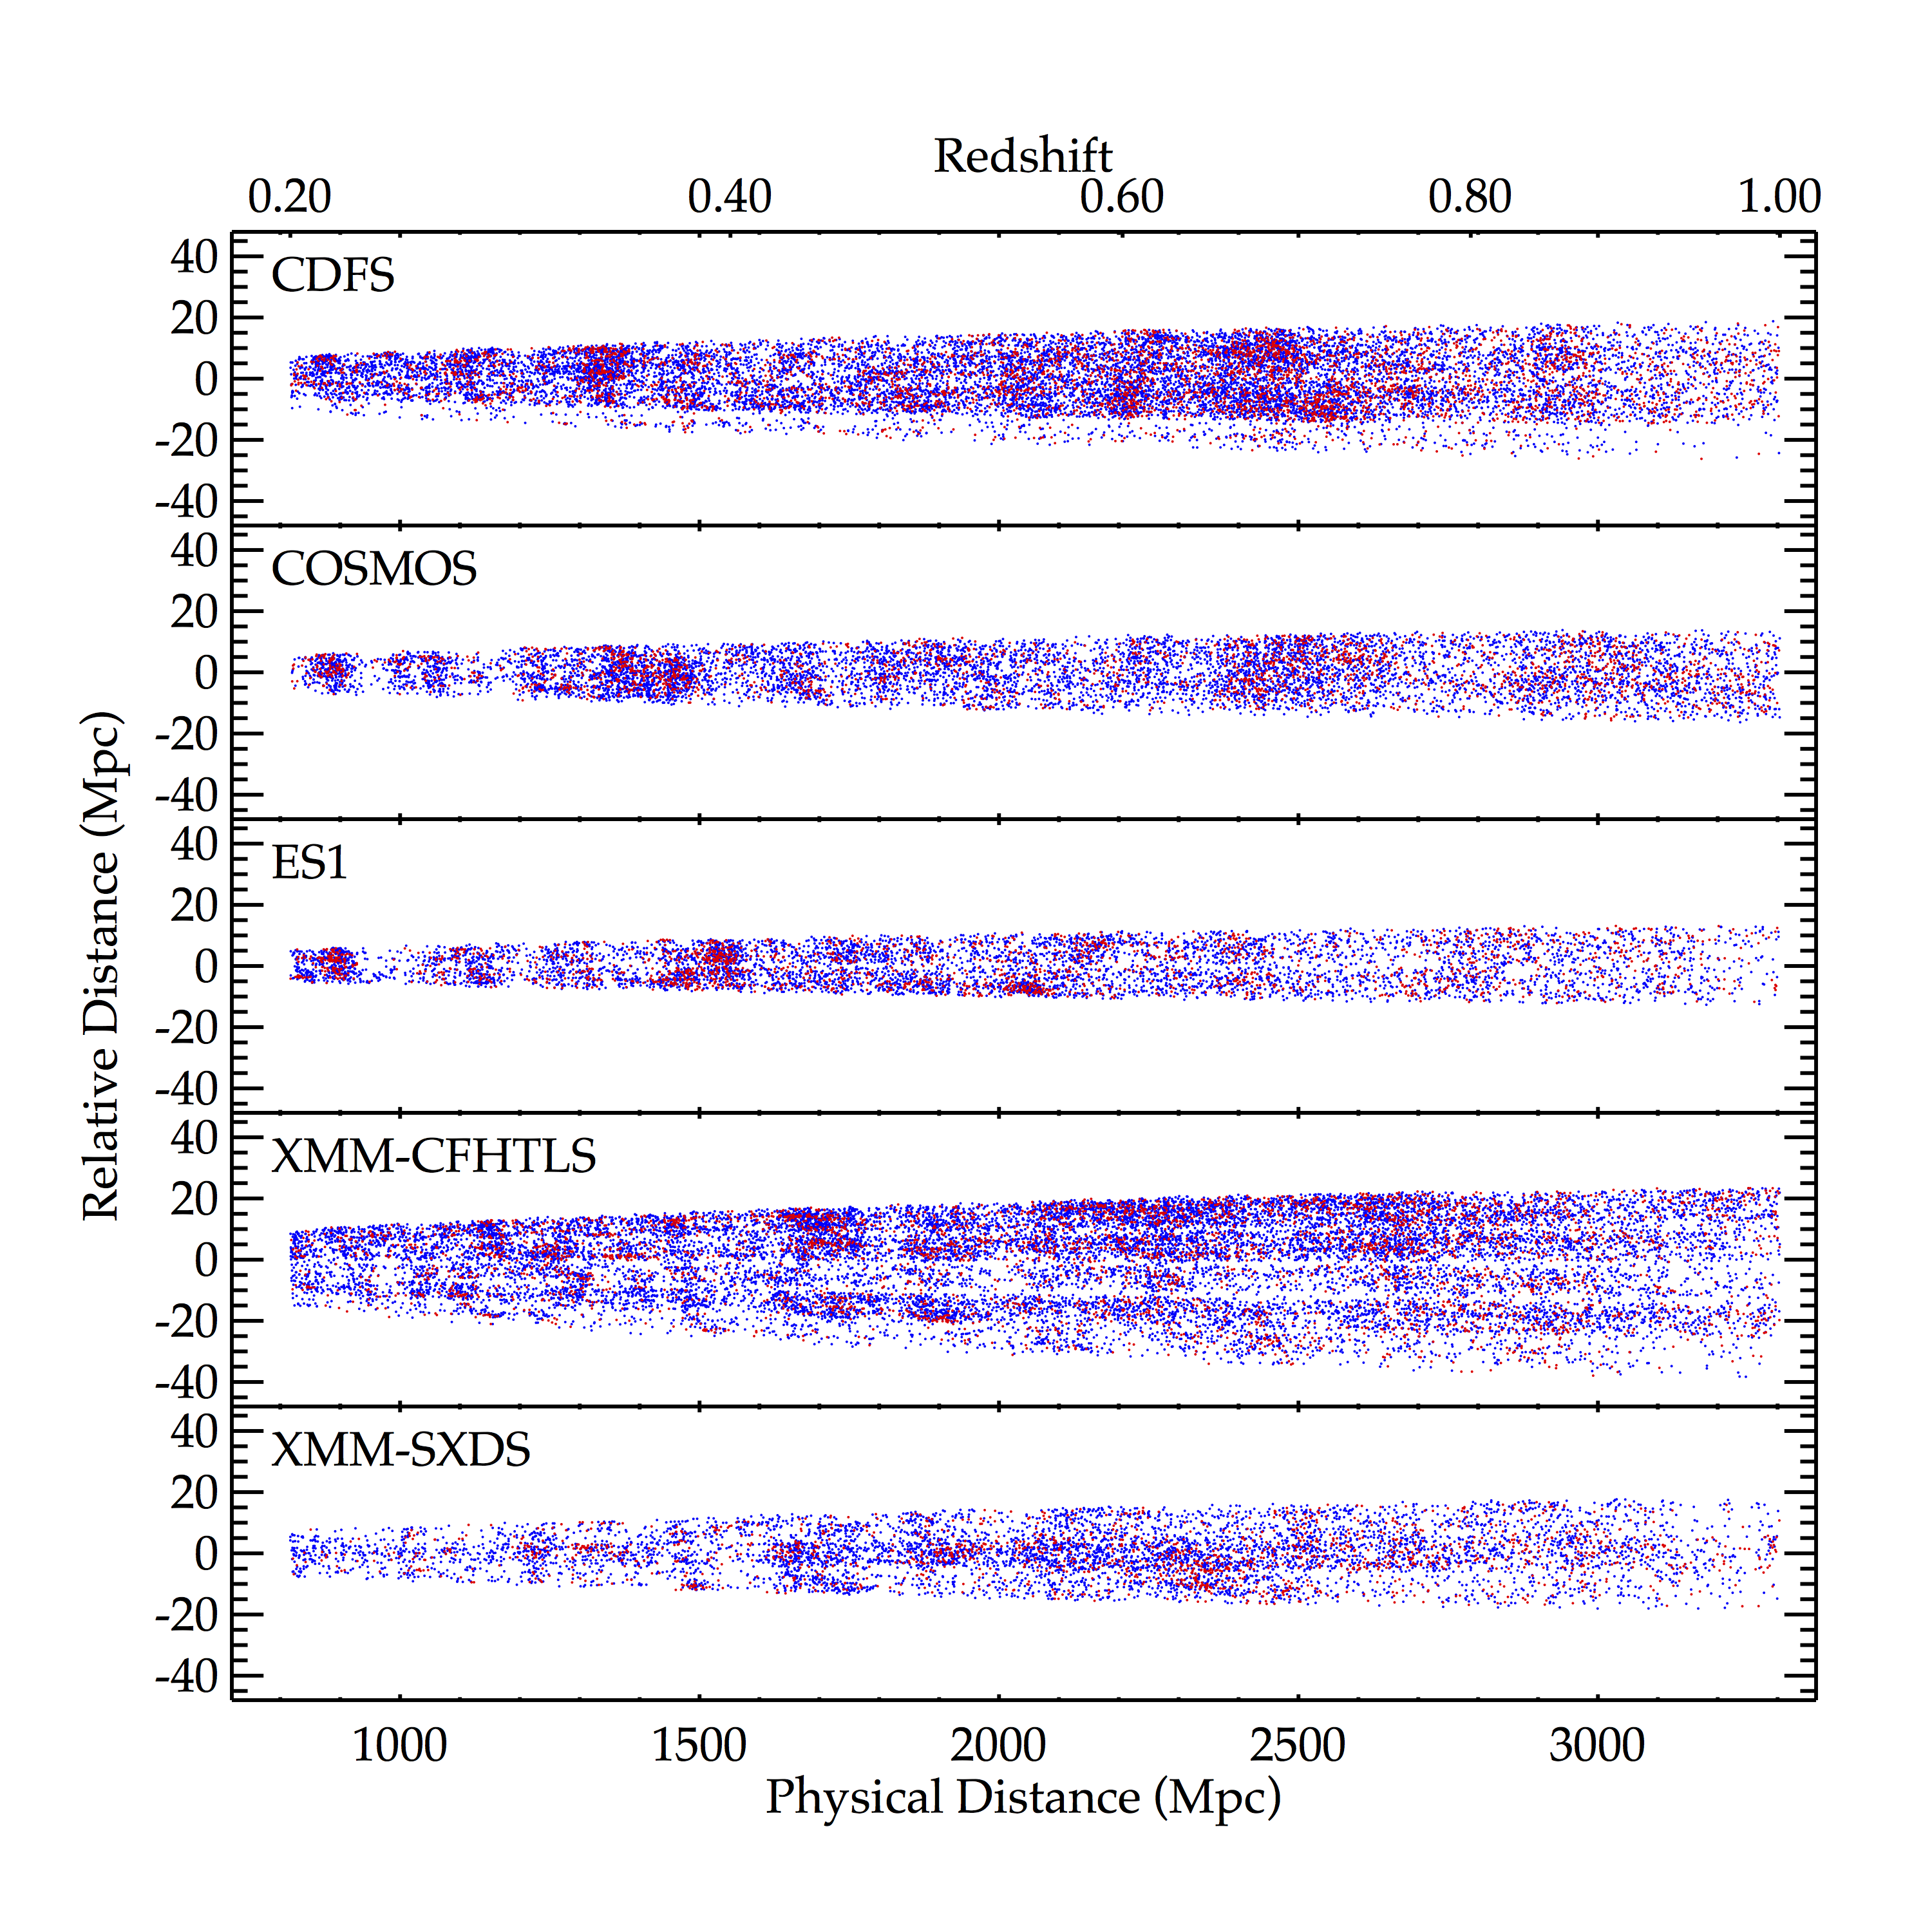
\includegraphics[width=0.9\textwidth,natwidth=600,trim={0.2in 0.5in 0.4in 0.6in},clip]{figures/cone_diagrams.png}}
  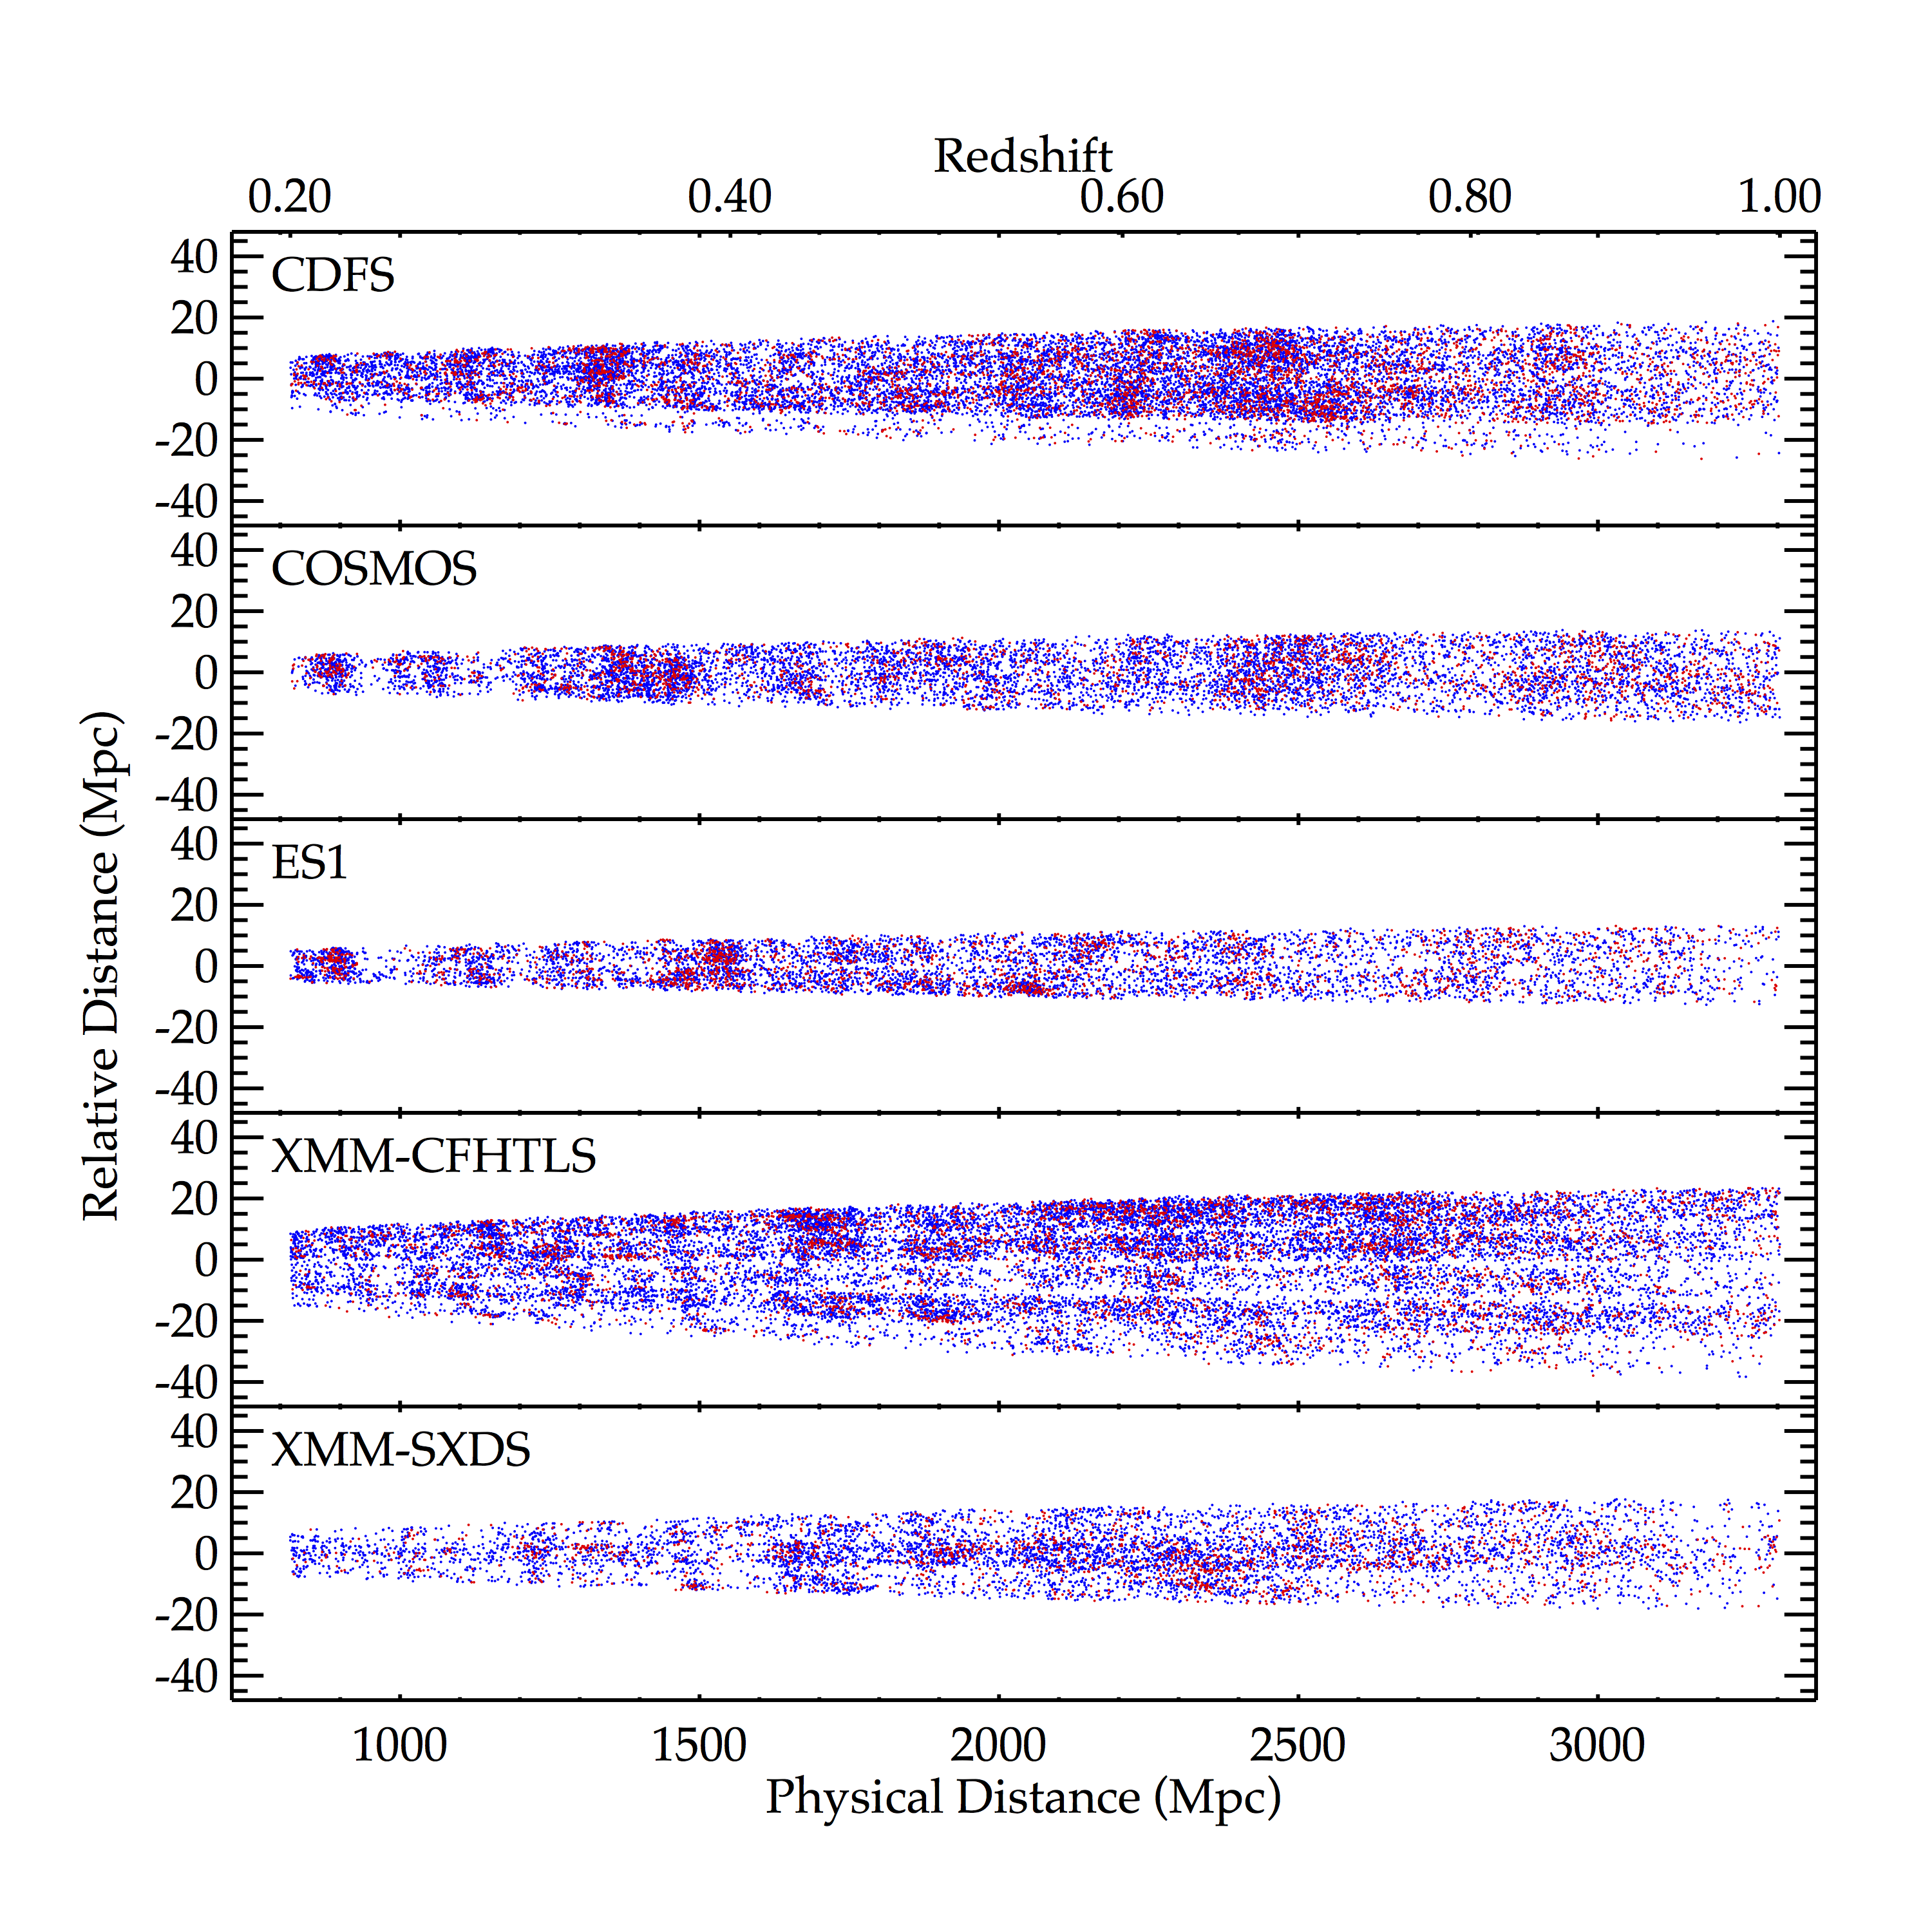
\includegraphics[width=0.9\textwidth,natwidth=600,trim={0.2in 0.5in 0.4in 0.6in},clip]{figures/cone_diagrams.png}
  \caption{Redshift space distributions of PRIMUS galaxies as a function of physical distance along the line-of-sight and right ascension 
(RA), relative to 
the median RA of the field.
%From top to bottom the corresponding fields are CDFS, COSMOS, ES1, XMM-CFHTLS, and XMM-SXDS.
Only galaxies with robust redshifts ${(Q \ge 3)}$ are shown.
Star-forming galaxies are shown in blue and quiescent galaxies in red (see~\S\ref{sec:SFQ}). Large scale differences in the observed 
density of galaxies, 
for example, as a function of RA, reflect the number of slitmasks and targeting density.
}
  \label{fig:cone_diagrams}
\end{figure*}

\subsection{Full Sample and Targeting Weights}\label{sec:targ_weight}
 

Objects in PRIMUS are classified as galaxies, stars, or broad-line active galactic nuclei by fitting the low-resolution spectra and multi-wavelength photometry 
for each source with an empirical library of templates.
The best-fit template defines both the redshift and the type of source.  
We exclude AGN from this study and keep only those objects defined as galaxies with robust redshifts {($Q\ge 3$)} in the redshift range {$0.2 < z < 1.0$}.
We also only keep galaxies with well defined targeting weights (these are termed ``primary'' galaxies in \citet{Coil11}; we do not use that naming here, to avoid 
confusion with our isolated primary sample defined below in \S\ref{sec:IPsample}).
These galaxies have a well understood spatial and targeting selection function, defined by both a density-dependent weight and a magnitude-dependent sparse-sampling 
weight, from which a statistically complete galaxy sample can be created.

PRIMUS targeting weights are described in detail in \citet{Coil11} and \citet{Cool13}.
% DENSITY-DEPENDENT WEIGHT
Briefly, density-dependent weights account for sources that PRIMUS could not target in dense survey regions, as galaxies are sufficiently clustered in the 
plane of
the sky to the PRIMUS flux limit that even two slitmasks per pointing could not target every galaxy below the magnitude limit in each field (as spectra would overlap on the detector). 
% MAGNITUDE-DEPENDENT "SPARSE SAMPLING WEIGHT"
Sparse-sampling weights are magnitude dependent and ensure that the PRIMUS target catalog is not dominated by the faintest objects within the survey flux limit. Sparse-sampling weights were used to randomly select roughly a third 
of galaxies in the faintest 0.5~mag interval above the primary sample 
targeting limit.
%Targets below the 100\% sampling limiting magnitude in each field (generally $i=22.5$) have a sparse-sampling weight of 1, while targets up to 0.5~mag fainter than 
%this limit (generally $22.5<i<23$) have a sparse-sampling weight of 0.3.
% REDSHIFT SUCCESS WEIGHT
A third, post-targeting weight \citep[detailed in][]{Cool13} accounts for the fact that not all PRIMUS spectra yielded reliable {($Q \ge 3$)} redshifts.
The average redshift success rate of the survey is a function of magnitude, declining from $>$75\% at {$i\le21$} to $\sim$30\% at the survey limit of $i=23$, and is not a strong function of color.  
Taken together, these three weights allow for the recovery of a statistically complete galaxy sample from the targeted sources with reliable redshifts.  

The full sample used here includes 60,071 galaxies with robust redshifts between $0.2<z<1.0$ and well understood selection weights, in the five fields discussed above.
Below we test the sensitivity of our results to these targeting and completeness weights.

\subsection{Stellar Mass and SFR Estimates}\label{sec:SFR}
 
Stellar masses and star formation rates (SFRs) of PRIMUS galaxies are obtained with SED fitting, a widely adopted method for estimating the physical properties of galaxies.
A complete description of the SED fitting process using \iSEDfit can be found in \citet{Moustakas13}, but we summarize the relevant points here.
\iSEDfit is a suite of routines written in the \IDL programming language that uses galaxy redshifts and photometry to compute the statistical likelihood of a large ensemble of model SEDs for each galaxy.
Model SEDs are generated using population synthesis models, and span a wide range of observed colors and physical properties (age, metallicity, star formation history, dust content, etc.).
\iSEDfit uses a Monte Carlo technique to randomly select values of model parameters from user-defined parameter distributions and compute a posterior probability distribution function (PDF).
PDFs of stellar mass and SFR are the found by marginalizing over all other parameters, and the median value of the marginalized PDF is taken as the best estimate of the stellar mass or SFR of each galaxy.
%Uncertainties are taken to be one quarter of the 2.3 to 97.7 percentile range of the PDF, equivalent to a $1\sigma$ uncertainty in the case of a Gaussian distribution.

\subsection{Identifying Star-forming and Quiescent Galaxies}\label{sec:SFQ}

We divide our sample into star-forming and quiescent galaxies based on each galaxy's position in the SFR\textendash stellar mass plane. 
%relative to the star formation (SF) sequence \citep{Noeske07}, the correlation between SFR and stellar mass exhibited by star-forming galaxies to at least {$z \sim 2$} \citep{Oliver10; Karim11}.
Figure~\ref{fig:SFR_vs_mass} shows SFR versus stellar mass in six redshift bins from ${z=0.2\textendash1}$ for the PRIMUS galaxy sample.
The dashed line (Eq.~\ref{eq:SFR}) in each panel traces the minimum of the bimodal galaxy distribution in that bin and is given by the following linear relation:
\begin{equation}\label{eq:SFR}
\log\,({\rm SFR}) = -1.29 + 0.65\,\log\,(\mass - 10) + 1.33\,(z - 0.1)
\end{equation}

\noindent where SFR has units of $\sfrunit$ and $\mass$ has units of $\msun$.
The slope of this line is defined by the slope of the star forming main sequence \citep{Noeske07} as measured in the PRIMUS dataset using \iSEDfit SFR and stellar mass estimates. 
Each galaxy is classified as star-forming or quiescent based on whether it lies above or below the cut defined by Equation~\ref{eq:SFR}, evaluated at the redshift of the galaxy.

\begin{figure}
  \centering
%  \fbox{\includegraphics[width=\linewidth,natwidth=600,trim={0.1in 0.1in 0.2in 0.6in},clip]{figures/SFR_vs_mass}}
  \includegraphics[width=\linewidth,natwidth=600,trim={0.1in 0.1in 0.2in 0.6in},clip]{figures/SFR_vs_mass}
%  \epsscale{1.1}
%  \epstrim{0.1in 0.1in 0.2in 0.6in}
%  \fbox{\plotone{figures/SFR_vs_mass}}
%  \plotone{figures/SFR_vs_mass}
  \caption{Star formation rate (SFR) versus stellar mass for PRIMUS galaxies in six redshift bins from ${z=0.2\textendash1}$.
Galaxies in our sample are classified as star-forming or quiescent according to whether they lie above or below the dashed line, respectively.
This line runs parallel to the star forming main sequence, traces the minimum in the galaxy SFR bimodality, and evolves with redshift according to Equation~\ref{eq:SFR}.
}
  \label{fig:SFR_vs_mass}
\end{figure}


\subsection{Isolated Primary Sample}\label{sec:IPsample}

In order to measure the galactic conformity signal, we must first identify isolated galaxies around which to search for the signal.
We follow \citet{Kauffmann13}, who selected in SDSS a volume-limited sample of galaxies with $\log\,\mstar>9.25$ and $0.017<z<0.03$.  They then defined ``central" galaxies of stellar mass $\mstar$ as those in their sample with no other galaxy with stellar mass greater than $\mstar/2$ within a projected radius of 500~kpc and with velocity difference less than 500~\kms.  Any galaxy in the full sample (defined above) is considered an isolated primary (IP) if there are no other galaxies
(i) within a projected physical distance of 500~kpc from the IP candidate,
(ii) within ${\pm 2.0\,\sigma_{z}\,(1 + z_{\rm IP})}$ in redshift space from the IP candidate (this includes as many true neighbors as possible while simultaneously minimizing interlopers and integrates over peculiar velocities), and
(iii) with stellar mass greater than half the stellar mass of the IP candidate.
Additionally, IPs can be neighbors of other IPs, and all galaxies can be a neighbor of multiple IPs. 

It is possible for galaxies near the edge of the survey area to be incorrectly classified as isolated if they have a sufficiently massive neighbor within a projected physical distance of 500~kpc that lies outside the survey area.
This could lead to contamination of our IP samples.
To test for this potential effect we visually inspected the distribution of IPs near the survey edges and concluded that false detections near edges do not significantly impact our IP sample, in that the spatial distribution of IPs does not rise substantially at the survey edges. 


{\bf(table 1 is out of order - need to fix that - also just say ``Matched IP sample stellar mass completeness limits'' and leave off the text about -3.7 - that information goes in the main text)}

\subsubsection{Stellar Mass Completeness Limits}\label{sec:mass_limit}

Because PRIMUS is a flux limited survey targeted in the $i$ band, galaxies with higher SFRs (i.e.~bluer galaxies) can be more easily detected at lower stellar mass than galaxies with lower SFR (i.e.~redder galaxies).
This introduces a bias towards star forming galaxies in the PRIMUS sample at lower stellar masses.
To account for this bias we define a stellar mass limit above which at least 95\% of all galaxies can be detected, regardless of their SFR.
This stellar mass completeness limit is a function of redshift, and also varies slightly between fields (due to the different photometry used for targeting in each field).
Details of the calculation of PRIMUS mass completeness limits can be found in \citet{Moustakas13}.
Briefly, we compute the stellar mass each galaxy would have if its apparent magnitude were equal to the survey magnitude limit, $\mlim$.  We then construct the cumulative distribution of $\mlim$ for the 15\% faintest galaxies in redshift bins of width 0.04, and calculate the minimum stellar mass that includes 95\% of the objects.  The limiting stellar mass versus redshift is fit with a separate quadratic polynomial for all, star-forming, and quiescent galaxies, and the fit is evaluated at the center of each redshift interval \citep[see][]{Moustakas13}.

In addition to the isolation criteria described above, all IPs must have stellar masses above the stellar mass completeness threshold in that field at the redshift of the galaxy. 
Of the 60,071 galaxies in the full sample, 14,888 star-forming and 6,847 quiescent galaxies meet the isolation and stellar mass completeness criteria to be IPs.


\subsubsection{Matching Stellar Mass and Redshift}\label{sec:IPsample_matching}

While our star-forming and quiescent IP populations are statistically complete (after applying the targeting and completeness weights), even above the stellar mass completeness limits the median stellar masses and redshifts of the two populations differ, as the stellar mass functions of star-forming and quiescent galaxies are different.
Figure~\ref{fig:IPhist_latefrac_vs_z} shows the redshift distributions of all star-forming (solid blue line) and quiescent (dashed red line) IPs, and the late-type fraction of all PRIMUS galaxies in the full sample as a function of redshift.
Our star-forming and quiescent IP populations have median stellar mass of $\log\,(\mstar/\msun)=10.44$ and 10.86, respectively, and median redshifts of $z=0.55$ and 0.60.

\begin{figure}
  \epsscale{1.1}
  \epstrim{0.1in 0.1in 0.5in 0.8in}
%  \fbox{\plotone{figures/IPhist_latefrac_vs_z}}
  \plotone{figures/IPhist_latefrac_vs_z}
  \caption{Top panel: Redshift histograms of all star-forming (solid blue line) and quiescent (dot-dashed red line) IPs.
Bottom panel: Late-type fraction of all PRIMUS galaxies in the full sample as a function of redshift. 
}
  \label{fig:IPhist_latefrac_vs_z}
\end{figure}

As discussed below, to compare the late-type fraction of neighbors around star-forming and quiescent IP galaxies we require the star-forming and quiescent IP samples to have the same stellar mass and redshift distributions.
To obtain these ``matched'' IP samples, we first apply to our IP samples an {\it upper} stellar mass cut derived from the PRIMUS stellar mass function (SMF, denoted as $\Phi$) for star-forming galaxies \citep{Moustakas13}.
This upper cut is required as there are fewer star-forming galaxies at high stellar mass ($\log\,(\mstar/\msun)>11$) than quiescent galaxies.
Therefore the high mass end of the star-forming galaxy SMF defines the limit of our matched IP samples.  
Specifically, we eliminate all IPs (both star-forming and quiescent) with stellar masses greater than the stellar mass at which 
${\log\,(\Phi \,/\, 10^{-4}\,\text{Mpc}^{-3}\,\text{dex}^{-1}) \le -3.7}$, interpolated at the redshift of each galaxy.
These upper mass limits are listed in Table~\ref{table:SMFlimit}.

%!TEX root = ../main.tex
\setlength{\tabcolsep}{0.1in}
\begin{deluxetable}{cc}
\tablewidth{0pc}
\tablecolumns{2}
\tablecaption{Matched IP sample stellar mass upper limits.
%$\log\,(\mlim/\msun)$ is the stellar mass in each redshift range where ${\log\Phi=-3.7}$.
%\tablenotemark{a}
\label{table:SMFlimit}
}
\tablehead{
%\multicolumn{1}{c}{} & \multicolumn{4}{c}{Area [deg$^2$]} & \multicolumn{6}{c}{Sample Size} \\
\colhead{Redshift Range} & \colhead{$\log\,(\mmax / \msun)$} }
\label{table:SMFlimit}
\startdata
$0.20-0.30$ & 11.154 \\
$0.30-0.40$ & 11.208 \\
$0.40-0.50$ & 11.255 \\
$0.50-0.65$ & 11.241 \\
$0.65-0.80$ & 11.308 \\
$0.80-1.00$ & 11.324 \\
%\hline \\[-2ex]
\enddata
%\tablenotetext{a}{$\mlim$ is the stellar mass in each redshift range where ${\log\Phi=-3.7}$.}
\end{deluxetable}


We then create a two-dimensional histogram of the stellar mass and redshift distribution of the remaining quiescent IP population, in bins of 0.2~dex in stellar mass and 0.05 in redshift.
For each of our five fields, in each bin we randomly select with replacement the same number of star-forming as there are quiescent IPs.
This selection is done separately in each field to account for field-to-field variations in the stellar mass and redshift distributions of the IP populations.
Our final matched IP sample contains 6,197 unique quiescent and 4,185 unique star-forming IPs.
Each star-forming IP is assigned a weight equal to the number of times it was randomly selected while matching the distribution of the quiescent IP sample.
The sum of all star-forming IP weights therefore equals the total number of unique quiescent IPs.
Figure~\ref{fig:IPsample_matched} shows the stellar mass and redshift distributions of all star-forming and quiescent galaxies in the full sample, as well as the stellar mass and redshift distributions of our final ``matched'' IP sample.

\begin{figure}
  \epsscale{1.1}
  \epstrim{0.6in 0.2in 0.2in 0.4in}
%  \fbox{\plotone{figures/matchedSamplePlot_allFields}}
  \plotone{figures/matchedSamplePlot_allFields}
  \caption{Stellar mass and redshift distribution for all star-forming (blue solid contours) and quiescent (red dashed contours) galaxies in the IP sample. 
Gray shaded contours show the distribution for the final ``matched'' star-forming and quiescent IP samples that have the same stellar mass and redshift distributions.
}
  \label{fig:IPsample_matched}
\end{figure}

%FIELD	MAX WGT	weight fraction = 1
%cdfs		6	0.658472
%XMM-CFHTLS	7	0.691321
%cosmos		6	0.651163
%es1		7	0.623077
%xmm-sxds	9	0.676667
